\section{künstliche Neuronale Netze}
\subsection{Multilayer Perceptron}

\begin{frame}
  \frametitle{Grundlagen}
  \begin{minipage}{0.5\textwidth}
   \begin{itemize}
     \item Eingabevektor $\vec{x}_l$
     \item Gewichtmatrix $\mathbf{W}^{\left( l \right)}$
     \item Aktivierungsfunktion $g^{\left( l \right)}$
     \item maAusgabevektor $\vec{y}^{(l)}$
   \end{itemize}
  \end{minipage}%
  \hfill%
  \begin{minipage}{0.5\textwidth}
    \begin{figure}
      \centering
      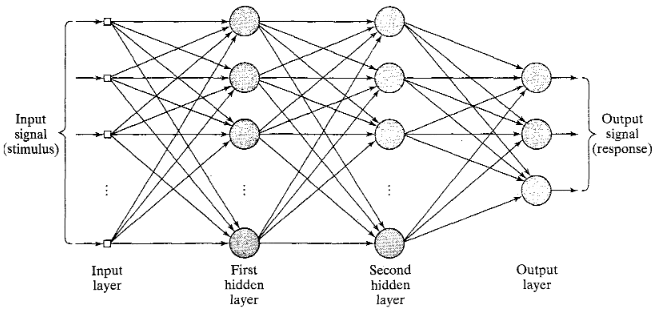
\includegraphics[width=\textwidth]{Plots/neuralnetworkhaykin.png}
      \caption{Quelle: Haykin, S.S., Neural Networks: A Comprehensive Foundation}
    \end{figure}
  \end{minipage}
\end{frame}

\begin{frame}
  \frametitle{mathematische Formulierung}
  \begin{block}{Definitionen}
    \begin{itemize}
      \item $\vec{y}^{\left( l \right)} = g^{\left( l \right)}
              \left( \bunderbrace{ \mathbf{W}^{\left( l \right)}
              \vec{x}^{\left( l \right)} + \vec{b}^{\left( l \right)}}
              {\coloneqq \vec{v}^{\left(l\right)} }  \right)$
      \item $g^{(l)}(\vec{x}^{(l)}) = g(\vec{x}^{(l)}) = ReLU \left( x \right) = \max \left ( 0,x \right)$
    \end{itemize}
  \end{block}
\end{frame}


\begin{frame}
  \frametitle{verschiedene Aktivierungsfunktionen}
  \begin{figure}
    \centering
    \includegraphics[width=0.8\textwidth]{Plots/Aktivierungsfunktionen.pdf}
  \end{figure}
\end{frame}

\subsection{Lernen und Fehlerrückführung}
\begin{frame}
  \frametitle{Ablauf des Lernalgorithmus}
  \begin{enumerate}
    \item Hinführung: Vorhersagewert $\vec{y}^{(l)}$, richtiger Wert $\vec{d}^{(l)}$
    \item Mean-squared-error (MSE) $\epsilon(n)$
    \item Fehlerrückführung: $\Delta w_{ij}^{\left( l \right)}\left(n\right)$
  \end{enumerate}
   \begin{block}{MSE, Gradientenabstiegsverfahren}
      \begin{itemize}
        \item $\epsilon \left ( n \right) = \frac{1}{2} \left( \vec{d}^{\left( l \right)}\left( n \right) -  \vec{y}^{\left( l \right)}\left( n \right)\right)^2$
        \item $\Delta w_{ij}^{\left( l \right)}\left(n\right) = - \eta \, \frac{\partial \epsilon\left(n\right)}{\partial w_{ij}^{\left( l \right)}\left(n\right) }$
      \end{itemize}
   \end{block}
\end{frame}

\begin{frame}
   \frametitle{Anpassung des Gradientenabstiegsverfahrens}
   \begin{itemize}
     \item kleine Lernrate: langsame Konvergenz
     \item große Lernrate: \enquote{Zig-Zagging}
     \item Impulskonstante $\alpha$
   \end{itemize}
   \begin{block}{Gradientenabstiegsverfahren mit Impulsterm}
      \begin{itemize}
        \item $\Delta w_{ij}^{\left( l \right)}\left(n\right) = - \eta \, \frac{\partial \epsilon\left(n\right)}{\partial w_{ij}^{\left( l \right)}\left(n\right) } + \alpha \Delta w_{ij}^{\left( l \right)}\left(n-1\right) $
      \end{itemize}
   \end{block}
\end{frame}

\begin{frame}
  \frametitle{Lern-Modi}
  \begin{itemize}
    \item Stochastic-Mode
    \item Batch-Mode
    \item Mini-Batch-Mode
  \end{itemize}
  \begin{block}{Gewichtsanpassung im Mini-Batch-Mode}
    \begin{itemize}
      \item $\Delta w_{ij}^{\left( l \right)}\left(n + 1\right) = \alpha \, w_{ij}^{\left( l \right)}\left(n + 1\right)
         + \eta \, \delta_j^{\left( l \right)}\left(n \right) \, y_i^{\left( l-1 \right)}\left(n \right)$
      \item $\delta_{j}^{\left( l \right)}\left(n \right) =
            \begin{dcases*}
              \left( d_j \left( n \right) - y_j^{\left( L \right)} \left(n \right) \right) \, g'\left( v_j^{\left(L \right)}\right)
              ,& \small{$j$-tes Perzeptron in Ausgabeschicht $L$}\\
              g'\left( v_j^{\left(l \right)}\right) \sum_{k} \delta_k^{\left(l+1\right)}\left(n\right) w_{kj}^{\left(l+1\right)}\left(n\right)
              ,& \small{$j$-tes Neuron in versteckter Schicht $l$}
            \end{dcases*}$
    \end{itemize}
  \end{block}

\end{frame}


\subsection{Trainieren des Neuronalen Netzes}

\begin{frame}
  \frametitle{Aufbau eines einfachen Modells}
  \begin{minipage}{0.5\textwidth}
    \begin{figure}
      \centering
      \includegraphics[width=\textwidth]{Plots/model_plot.pdf}
    \end{figure}
  \end{minipage}%
  \hfill%
  \begin{minipage}{0.5\textwidth}
    \begin{enumerate}
      \item input layer - 99 Neuronen
      \item hidden layer - 20 Neuronen
      \item hidden layer - 10 Neuronen
      \item output layer - 1 Neuron
    \end{enumerate}
  \end{minipage}
\end{frame}

\begin{frame}
  \frametitle{Overfitting und Early Stopping}
  \begin{figure}
    \centering
    \includegraphics[width=0.8\textwidth]{Plots/MSE.pdf}
  \end{figure}
\end{frame}

\begin{frame}
  \frametitle{Early Stopping - aber wann?}
  \begin{figure}
    \centering
    \includegraphics[width=0.8\textwidth]{Plots/MSE150k.pdf}
  \end{figure}
\end{frame}

\begin{frame}
  \frametitle{Graphische Veranschaulichung zur Validierung}
  \begin{figure}
    \centering
    \includegraphics[width=0.8\textwidth]{Plots/mlp_test_new.pdf}
  \end{figure}
\end{frame}

\begin{frame}
  \frametitle{Hyperparameteroptimierung im Vergleich}
  \begin{minipage}{0.5\textwidth}
    \begin{figure}
      \centering
      \includegraphics[width=\textwidth]{Plots/MSEOpt.pdf}
    \end{figure}
  \end{minipage}%
  \hfill%
  \begin{minipage}{0.5\textwidth}
      \begin{itemize}
        \item Konfigurationsraum \\
        \begin{enumerate}
          \item Anzahl Neuronen in den versteckten Schichten
          \item Dropoutlayer zwischen den versteckten Schichten
        \end{enumerate}
        \item Tree-Structured Parzen Estimator (TPE), jeweils 1000 Epochen
      \end{itemize}
  \end{minipage}
  \begin{minipage}{\textwidth}
     \begin{enumerate}
       \item input layer - 99 Neuronen
       \item hidden layer - 20 Neuronen
       \item dropout layer - 33.8 \%
       \item hidden layer - 8 Neuronen
       \item output layer - 1 Neuron
     \end{enumerate}
  \end{minipage}

\end{frame}

\begin{frame}
  \frametitle{Einfluss mehrerer Aufnahmen}
  \begin{minipage}{0.7\textwidth}
    \begin{figure}
      \centering
      \includegraphics[width=\textwidth]{Plots/multiple.pdf}
    \end{figure}
  \end{minipage}%
  \hfill%
  \begin{minipage}{0.3\textwidth}
    \begin{figure}
      \centering
      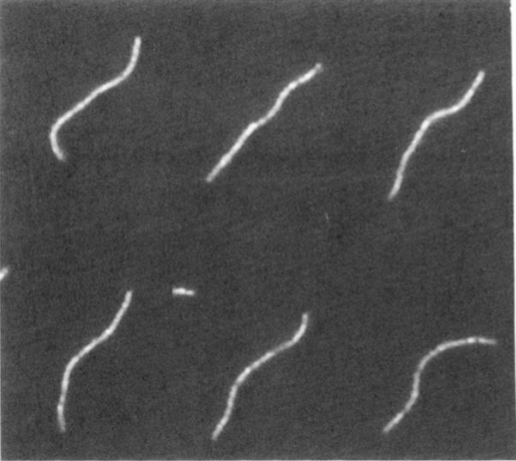
\includegraphics[width=\textwidth]{Plots/f-aktin.png}
      \caption{Quelle: \url{https://link.aps.org/doi/10.1103/PhysRevE.48.R1642}}
    \end{figure}
  \end{minipage}
\end{frame}

%\begin{frame}
%       \begin{tabular}{cl}
%         \begin{tabular}{c}
%           \includegraphics[width=0.5\textwidth]{Plots/Aktivierungsfunktionen.pdf}
%           \end{tabular}
%           & \begin{tabular}{l}
%             \parbox{0.5\linewidth}{%  change the parbox width as appropiate
%             $\text{ReLU}(x) = \text{max}(0,x)$
%                                    }
%             \end{tabular}  \\
%         \end{tabular}
%\end{frame}
